%*******************************************************************************
%****************************** Second Chapter *********************************
%*******************************************************************************

\chapter{Marco teórico} \label{ch:theory}


\ifpdf
    \graphicspath{{Chapter2/Figs/Raster/}{Chapter2/Figs/PDF/}{Chapter2/Figs/}}
\else
    \graphicspath{{Chapter2/Figs/Vector/}{Chapter2/Figs/}}
\fi

En este capítulo se presentan los requerimientos y la teoría de base necesaria para el desarrollo de este trabajo de tesis. El mismo se encuentra dividido en seis secciones. La primer sección trata sobre los requerimientos necesarios que se deben cumplir para para obtener el objetivo. En la segunda se discuten las diferencias entre los principales tipos de radares, continuos y pulsados. Luego se presenta la problemática de ambigüedades en rango para ambos grupos. A continuación se resumen las características de cada geometría de antena, en particular se detallan monopolos y dipolos. A su vez se introduce el concepto de polarización asociado a la matriz de polarización cuyos componentes se desean conocer. En la quinta se introduce el concepto de parámetros S. Por último, en la última sección se detalla el procesamiento que se le debe aplicar a la señal recibida para un radar FMCW.

\section{Requerimientos}

El objetivo del trabajo de tesis, o requerimiento L0, es poder medir la matriz de dispersión de cuerpos con una cierta incertidumbre aceptable a una distancia del orden de los metros. Dicha propiedad es importante dado que la misma es utilizada para distintos tipos de aplicaciones. Las principales son el estudio de hielo polar, mareas oceánicas, mapeo del suelo o subsuelo, humedad del suelo y ecología forestal \cite{Curlander}.

La matriz de dispersión está definida por la ecuación \ref{eq:backscatteringMatrix}. Cada elemento de la matriz es un número complejo que indica la relación entre la señal reflejada e incidente en las distintas combinaciones de polarizaciones, horizontal (H) y vertical (V). La nomenclatura utilizada es la unión entre polarizaciones incidentes y reflejadas respectivamente.

\begin{equation} \label{eq:backscatteringMatrix}
  \bm{\sigma} = \begin{bmatrix} \bm{HH} & \bm{HV} \\ \bm{VH} & \bm{VV} \end{bmatrix}
\end{equation} 

Para cumplir con dicho objetivo el radar debe poder determinar el desfase y la atenuación que el blanco induce sobre la señal en las diferentes combinaciones de polarizaciones. De esta forma se definen los requerimientos \ref{req:l1_gain}, \ref{req:l1_phase} y \ref{req:l1_pol}. En la figura \ref{fig:requirements} se muestran todos los requerimientos de nivel alto, medio y bajo.

\begin{figure}[H]
  \centering
  \begin{tabular}{@{} l @{} c @{} l @{} c @{} l @{}}

  \begin{tabular}[t]{|@{}p{4.6cm}@{}|}
    \hline
    \centering \textbf{Requerimientos L0} \tabularnewline
    \hline
    \tabularnewline

    \begin{enumerate}[label=L0.\arabic*, nosep]
      \req{Matriz de dispersión} \label{req:l0}
    \end{enumerate} \tabularnewline

    \hline
  \end{tabular} &

  \begin{tabular}[t]{@{}c@{}}
    \tabularnewline
    \tabularnewline
    \tabularnewline
    $\Rightarrow$ \tabularnewline
  \end{tabular} &

  \begin{tabular}[t]{|@{}p{4.6cm}@{}|}
    \hline
    \centering \textbf{Requerimientos L1} \tabularnewline
    \hline

    \begin{enumerate}[label=L1.\arabic*, nosep]
      \req{Clase de Radar} \label{req:l1_radarType}
      \req{Polarización} \label{req:l1_pol}
      \req{Distancia} \label{req:l1_distance}
      \req{Medición Ganancia} \label{req:l1_gain}
      \req{Medición Fase} \label{req:l1_phase}
    \end{enumerate} \tabularnewline

    \hline
  \end{tabular} &

  \begin{tabular}[t]{@{}c@{}}
    \tabularnewline
    \tabularnewline
    \tabularnewline
    $\Rightarrow$ \tabularnewline
  \end{tabular} &
  
  \begin{tabular}[t]{|p{4.6cm}|}
    \hline
    \centering \textbf{Requerimientos L2} \tabularnewline
    \hline

    \begin{enumerate}[label=L2.\arabic*, nosep]
      \req{Frecuencia central} \label{req:l2_f0}
      \req{Ancho de banda} \label{req:l2_bw}
      \req{Potencia de transmisión} \label{req:l2_txPower}
      \req{Período Pulso} \label{req:l2_pulseT}
      \req{Ciclo Trabajo} \label{req:l2_dutyCycle}
      \req{Modulación} \label{req:l2_mod}
      \req{Filtro} \label{req:l2_filter}
      \req{Cantidad de Antenas} \label{req:l2_antQuantity}
      \req{Tipo Antena} \label{req:l2_antenna}
      \req{Polarizacion} \label{req:l2_polarization}
      \req{Altura de pesca} \label{req:l2_pescaLength}
      \req{Diámetro de cavidad} \label{req:l2_cavity}
      \req{Distancia pesca a pared} \label{req:l2_cavityDistance}
      \req{Peso del radar} \label{req:l2_weight}
    \end{enumerate} \tabularnewline

    \hline
  \end{tabular} \tabularnewline

  \end{tabular}
  \caption{Requerimientos de alto, medio y bajo nivel de construcción del radar.}
  \label{fig:requirements}
\end{figure}

A continuación se detallan los requerimientos ilustrados en la figura \ref{fig:requirements}. Los mismos se definen a lo largo del desarrollo del presente trabajo de tesis.

\subsection{Requerimientos de alto nivel}

Dichos requerimientos reflejan el objetivo al que se quiere llegar.
\begin{description}
  \item[\ref{req:l0}] El radar debe ser capaz de determinar la matriz de dispersión de cuerpos a una distancia menor a $\SI{20}{\meter}$ metros.
\end{description}


\subsection{Requerimientos de nivel medio}

Dichos requerimientos definen la solución propuesta para cumplir con el requerimiento de alto nivel.

\begin{description}
  \item[\ref{req:l1_radarType}] El radar debe ser del tipo FMCW.
  \item[\ref{req:l1_pol}] El radar debe ser capaz de transmitir y recibir en ambas polarizaciones, vertical y horizontal.
  \item[\ref{req:l1_distance}] El radar debe ser capaz de determinar la distancia al cuerpo iluminado.
  \item[\ref{req:l1_gain}] El radar debe ser capaz de determinar la ganancia del cuerpo iluminado con una incertidumbre no mayor a $\SI{0.2}{\dB}$.
  \item[\ref{req:l1_phase}] El radar debe ser capaz de determinar el desfase del cuerpo iluminado con una incertidumbre no mayor a $\SI{30}{\deg}$.
\end{description}


\subsection{Requerimientos de bajo nivel}


\mynote{consumo, centro de masa, potencia consumida para la autonomía, crosstalk}
Dichos requerimientos detallan las propiedades de los subsitemas de la solución propuesta para cumplir con los requerimientos de medio y alto nivel.

\begin{description}
  \item[\ref{req:l2_f0}] La frecuencia central de la señal transmitida debe ser igual a $\SI{1245}{\MHz}$.
  \item[\ref{req:l2_bw}] El ancho de banda de la señal transmitida debe ser de $\SI{300}{\MHz}$.
  \item[\ref{req:l2_txPower}] La potencia de transmisión debe ser de $\SI{12}{\dBm}$.
  \item[\ref{req:l2_pulseT}] El período de la señal transmitida no debe ser menor a $\SI{13.5}{\mu\sec}$.
  \item[\ref{req:l2_dutyCycle}] El ciclo de trabajo de la señal transmitida debe poder ser configurable, de $\SI{0.05}{\percent}$ a $\SI{99.95}{\percent}$ para realizar ensayos futuros comparando distintas modulaciones.
  \item[\ref{req:l2_mod}] La modulación debe ser del tipo triangular o sinusoidal para realizar ensayos futuros comparando distintas modulaciones.
  \item[\ref{req:l2_filter}] El filtro pasa bajos del radar debe tener una frecuencia de corte superior igual a $\SI{20}{\kHz}$.
  \item[\ref{req:l2_antQuantity}] El radar debe tener dos antenas, una transmisora y una receptora.
  \item[\ref{req:l2_antenna}] Las antenas son del tipo monopolo dentro de una cavidad.
  \item[\ref{req:l2_polarization}] Las antenas deben ser polarimétricas.
  \item[\ref{req:l2_pescaLength}] La longitud de cada monopolo dentro de las cavidades debe ser igual a $\SI{3}{\centi\meter}$.
  \item[\ref{req:l2_cavity}] El diámetro de la cavidad de la antena debe ser mayor a $\SI{7.64}{\centi\meter}$ y menor a $\SI{11.2}{\centi\meter}$.
  \item[\ref{req:l2_cavityDistance}] La distancia entre la pesca y la pared de la cavidad debe ser igual a $\SI{4.39}{\centi\meter}$.
  \item[\ref{req:l2_weight}] El radar no debe pesar más de $\SI{1}{\kg}$.
\end{description}

A continuación se discute sobre las dos familias principales de radares para definir el que se utiliza en el presente trabajo.

\section{Onda continua versus pulsada}

La modulación de onda de los radares puede dividirse en dos clases principales, onda continua (CW) y pulsado.

Cuando es continua, el transmisor transmite continuamente una señal sin interrupción mientras el radar está operando. El receptor también opera continuamente. Como contraparte, en los radares pulsados, el transmisor emite una secuencia de pulsos de duración finita. Cuando esto ocurre, el receptor está encendido de forma tal que la señal del blanco iluminado puede detectarse.


\subsection{Onda pulsada}

Los Radares pulsados transmiten ondas electromagnéticas (EM) durante un corto tiempo, o pulso de ancho $\tau$, típicamente entre 0.1 a 10 micro segundos ($\si{\us}$), aunque a veces es de unos pocos nano segundos o tan largos como un mili segundo. Durante este tiempo, el receptor está aislado de la antena, o protegido dado que sus componentes son sensibles a la alta potencia de las ondas EM transmitidas. En dicho tiempo no se puede detectar ninguna clase de señal. Entre pulsos transmitidos, el receptor está conectado a la antena, permitiendo así recibir ondas EM, o ecos, que pueden haber sido reflejados desde objetos del ambiente. Al tiempo entre el inicio de dos pulsos transmitidos normalmente se la llama período entre pulsos (IPP) o intervalo de repetición entre pulsos (PRI). La forma de onda pulsada se muestra en la figura \ref{fig:pulsedWaveform} \cite{Richards2010}.

\begin{figure}
 \centering
 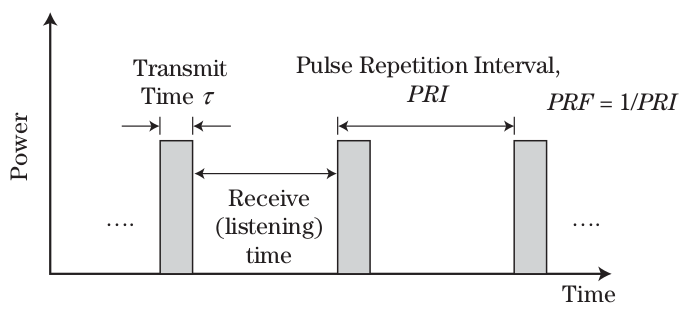
\includegraphics[width=10cm]{pulsedWaveform}
 \caption{Forma de onda de un radar pulsado \cite{Richards2010}.}
 \label{fig:pulsedWaveform}
\end{figure}


\subsection{Onda continua}

Generalmente este tipo de radares utilizan una configuración biestática, implicando que el transmisor se encuentre separado del receptor, para aumentar la aislación entre las antenas. Pero, como la aislación no es perfecta, utilizan baja potencia de transmisión. Por lo tanto, sólo son utilizados en aplicaciones de rangos cortos. Aunque hay sistemas complejos de radares de onda continua como iluminadores en sistemas de control de fuego, misiles semi activos, y rastreadores, también los hay con esquemas simples, aplicados en radares de velocidad, altímetros y sensores de proximidad \cite{Richards2010}. La figura \ref{fig:continuousWaveform} muestra un ejemplo de una modulación diente de sierra.

Dado que la transmisión es continua, la determinación del tiempo de ida y vuelta, del inglés round-trip time, de la señal electromagnética (EM) transmitida, por ende la distancia del blanco iluminado, debe realizarse cambiando las características de la señal. Por ejemplo modificando su frecuencia a través del tiempo. Esta técnica de modulación en frecuencia (FM) introduce una marca de tiempo en la onda EM, permitiendo así la determinación de la distancia al blanco.

\begin{figure}[H]
 \centering
 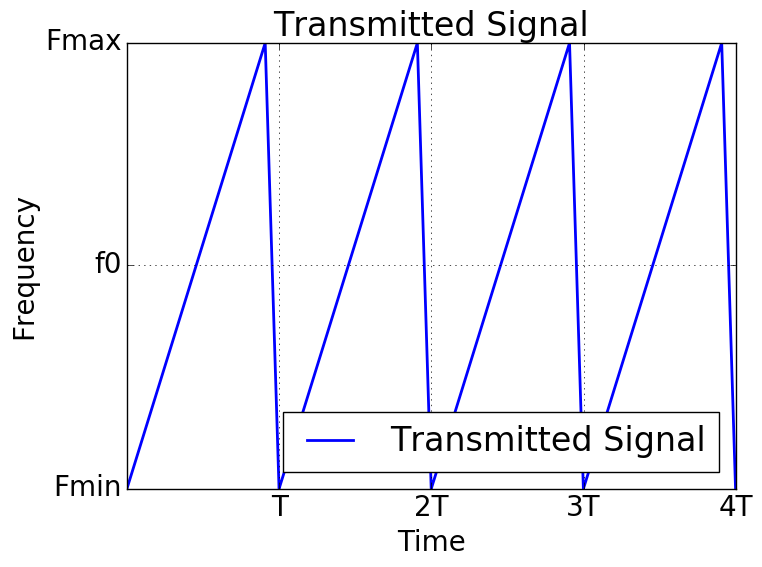
\includegraphics[width=8cm]{sawtoothSignal}
 \caption{Forma de onda de la señal transmitida por un radar FMCW.}
 \label{fig:continuousWaveform}
\end{figure}

En el presente trabajo de tesis, como se desea posicionar el cuerpo a una distancia del orden de los metros, se opta por utilizar este esquema de radares. Definiéndose de esta forma el requerimiento \ref{req:l1_radarType}.


\section{Ambigüedades en mediciones de rango} \label{sc:ambiguity}

Como la distancia a un cuerpo iluminado se mide determinando el tiempo de ida y vuelta entre la señal transmitida y el eco recibido, si dicho tiempo es mayor que el PRI, el sistema determina erróneamente dicha distancia. Este error es el llamado ambigüedad.

En la figura \ref{fig:ambiguity} se muestra un ejemplo de este efecto para un radar pulsado. Hay dos blancos, el primero a una distancia cercana y el segundo a una lejana, de tal forma, que el tiempo de ida y vuelta es mayor que el PRI. Se puede observar que el eco de la señal transmitida en el primer período del segundo blanco llega a la antena durante el tiempo de recepción del segundo período transmitido, logrando así un error en la estimación de la distancia a este blanco.

Para evitar tener ambigüedades, se debe incrementar el PRI lo suficiente para que todos los blancos estén dentro del máximo tiempo de ida y vuelta detectable.

\begin{figure}[H]
 \centering
 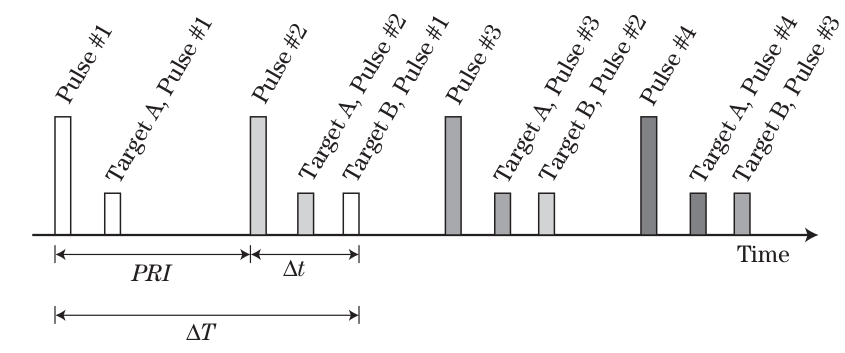
\includegraphics[width=10cm]{ambiguity}
 \caption{Ambigüedades en mediciones de rango en un radar pulsado \cite{Richards2010}.}
 \label{fig:ambiguity}
\end{figure}

En el caso de los radares FMCW, la determinación de la distancia está relacionada con la frecuencia de la señal a procesar y, dado que se transmite constantemente e independientemente de la posición en que estén los blancos iluminados, siempre habrá un solapamiento entre el pulso transmitido siguiente y la señal recibida del pulso anterior. En la figura \ref{fig:fmcwAmbiguity} se puede apreciar dicho solapamiento entre los tiempos T y T1. Como la señal a procesar es la multiplicación entre el pulso transmitido y recibido, la frecuencia recibida en el intervalo T y T1 varía a causa de la mezcla entre pulsos consecutivos, ver figura \ref{fig:modulationDelayed}.

Para evitar errores en el cálculo de la estimación en la frecuencia, se puede aplicar un retraso en la señal a procesar, evitando tomar las muestras correspondientes al solapamiento entre pulsos o se puede transmitir interrumpiendo durante un tiempo equivalente o superior al máximo tiempo de ida y vuelta de la señal admitido \cite{Varavin2007a}. Por último, para disminuir errores en dicho cálculo se aumenta la duración del tiempo T, aumentando el ancho de banda o disminuyendo la pendiente de la rampa de la señal modulada.

\begin{figure}[H]
  \centering
  \begin{subfigure}[t]{0.49\textwidth}
    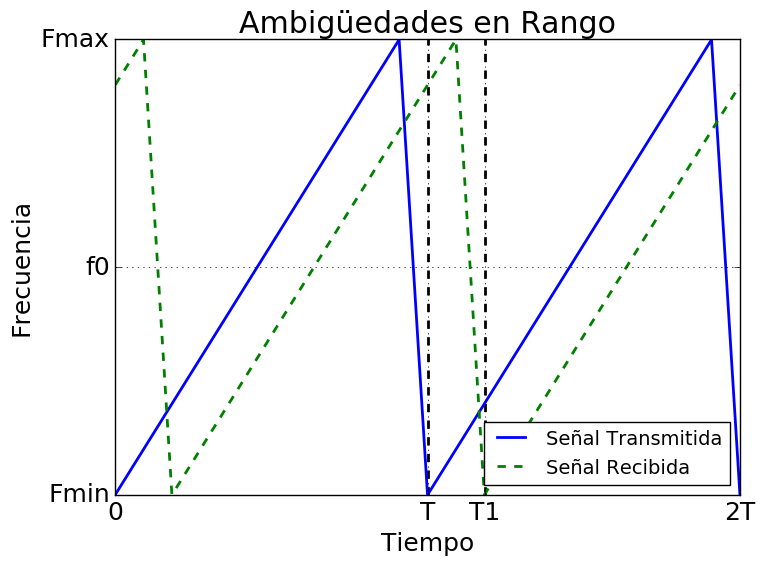
\includegraphics[width=7.5cm]{FMCWambiguity}
    \caption{Señal transmitida y recibida en función del tiempo}
    \label{fig:fmcwAmbiguity}   
  \end{subfigure}
  \begin{subfigure}[t]{0.49\textwidth}
    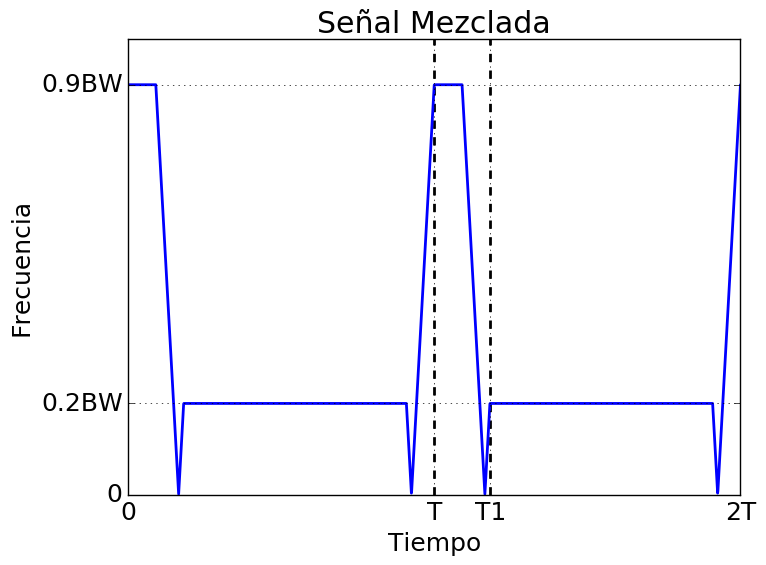
\includegraphics[width=7.5cm]{receivedFrequency}
    \caption{Frecuencia recibida de la señal a procesar.}
    \label{fig:modulationDelayed}
  \end{subfigure}             
  \caption{Ambigüedades en un radar FMCW.}
\end{figure}

\section{Antenas}

Una antena es definida como la estructura de transición entre el espacio libre y un dispositivo guía, como se muestra en la 
figura \ref{fig:antenna}. El dispositivo guía o línea de transmisión puede ser un cable coaxial o un tubo hueco (guía de 
onda), el cual es utilizado para transportar energía electromagnética desde la fuente de transmisión a la antena, o desde la 
antena al receptor. En el primer caso sería una configuración de antena transmisora y en el segundo, receptora \cite{Balanis2012}.
\begin{figure}[H]
 \centering
 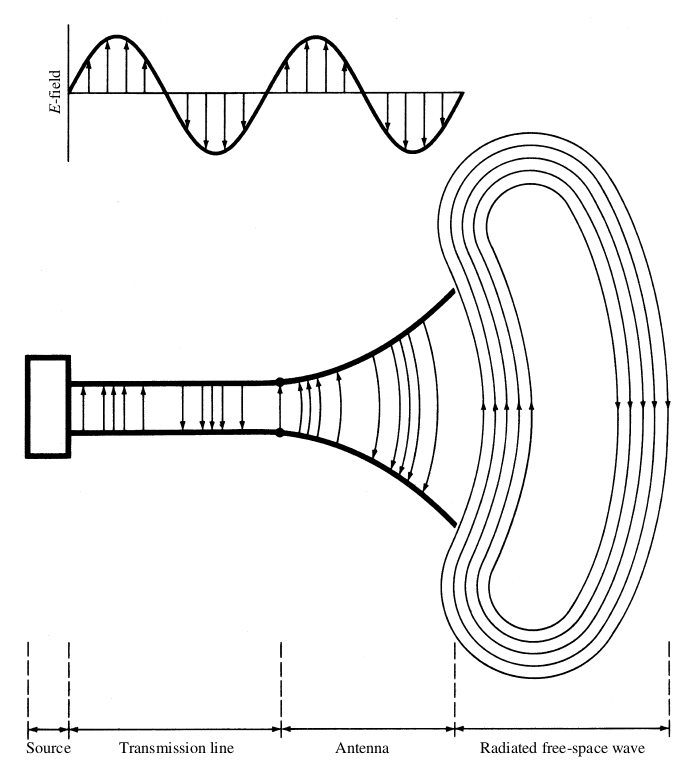
\includegraphics[width=10cm]{antenna}
 \caption{Antena como un dispositivo de transmisión \cite{Balanis2012}.}
 \label{fig:antenna}
\end{figure}

Hay una amplia variedad de antenas en la actualidad, en la tabla \ref{tab:type_antennas} se puede observar una agrupación 
simplificada.

\begin{table}[H]
  \caption{Características de cada grupo principal de antenas}
  \footnotesize
  \centering
  \begin{tabular}{l p{12.5cm}}
  \toprule
  \textbf{Tipo Antena} & \textbf{Características} \tabularnewline
  \midrule
  Cable & Son el tipo de antenas más utilizados porque se las puede en autos, edificios, barcos, sistemas aeroespaciales. Hay distintas formas de estas antenas, como monopolos, dipolos, lazos y hélices o alguna otra configuración. Los usos más comunes de los monopolos son para radios AM/FM y walkie talkies; de los dipolos son para antenas de canales de tv VHF o antena de televisión analógico; y de lazos son para receptoras de canales UHF de tv o receptores de AM \cite{Balanis2012}. \tabularnewline

  Apertura & Son el principal tipo de antenas direccionales utilizadas en frecuencias microondas. Consisten en una antena
  del tipo dipolo o Lazo junto a una estructura que guía las ondas en una dirección determinada. Este tipo de antenas son muy utilizadas en el ámbito aéreo y espacial dado que se pueden empotrar en la superficie del avión o satélite. A su vez, se los puede cubrir con un material dieléctrico para protegerlos de las condiciones ambientales \cite{Balanis2012}. \tabularnewline
  
  Microstrip & Consisten en un patch metálico sobre un sustrato. Dicho patch puede tomar distintas formas, aunque, la rectangular y circular son las más populares dada su facilidad de fabricación y por sus características de radiación, como por ejemplo la baja radiación en la polarización cruzada. Este tipo de antenas son simples, de bajo costo de fabricación, son mecánicamente robustas si se las monta en superficies rígidas y muy versátiles en términos de frecuencias de resonancia, polarización, diagramas de radiación e impedancias. Son muy utilizadas en aplicaciones aeroespaciales y celulares \cite{Balanis2012}. \tabularnewline

  Conjunto & Muchas aplicaciones requieren características de radiación que pueden no ser alcanzables con un único elemento sino que por un conjunto de elementos en una distribución eléctrica y geométrica determinada. La distribución adoptada afecta en distintos aspectos al diagrama de radiación. Algunos usos son Transmisión de canales de televisión en VHF, detección de misiles, comunicaciones satelitales \cite{Balanis2012}. \tabularnewline
  
  Reflectores & Estas antenas son utilizadas para comunicaciones a largas distancias, para transmitir y recibir señales que tienen que recorrer kilómetros. Un estilo muy común de este tipo de antenas es el reflector parabólico, el diámetro máximo construido es de $\SI{305}{\meter}$, necesario por la gran ganancia requerida para transmitir o recibir señales a miles de kilómetros. Otro tipo de reflector no tan común como la parábola es el corner reflector \cite{Balanis2012}. \tabularnewline

  Lentes & Son utilizadas principalmente para transformar energía divergente en ondas planas, de esta forma se previene  transmisión en direcciones indeseadas. Se pueden utilizar en casi las mismas aplicaciones que los reflectores parabólicos, especialmente en altas frecuencias. Para bajas frecuencias no son utilizadas dado que sus dimensiones y peso se tornan inmanejables \cite{Balanis2012}. \tabularnewline
  \bottomrule 
  \end{tabular}
  \label{tab:type_antennas}
\end{table}

Por la simplicidad de construcción, en la presente tesis se opta por utilizar el tipo de antena monopolo, de esta forma se desprende el requerimiento \ref{req:l2_antenna}. A continuación se detalla este tipo de antenas comparándolo con su contraparte, el dipolo.


\subsection{Monopolos y Dipolos}

Un monopolo es un dipolo que ha sido dividido a la mitad de su punto de alimentación central y es alimentado contra un plano de tierra, el cual actúa como un estilo de espejo eléctrico \cite{arrl2007}. La figura \ref{fig:monopoles} compara un dipolo de $\frac{\lambda}{2}$ con un monopolo de $\frac{\lambda}{4}$ de longitud. La antena imagen, para el monopolo, está representada con una línea punteada debajo del plano de tierra. La misma forma la segunda mitad de la antena, transformando funcionalmente al monopolo en un dipolo.

\begin{figure}
 \centering
 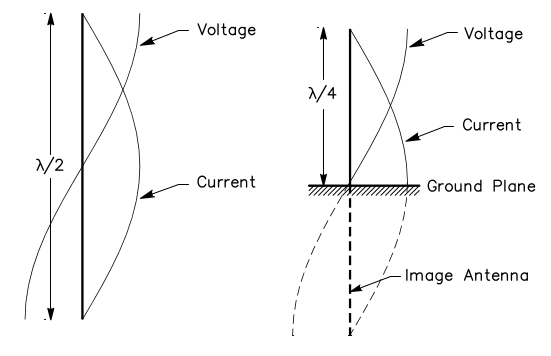
\includegraphics[width=10cm]{monopoleVsDipole}
 \caption{Un dipolo de longitud $\frac{\lambda}{2}$ y su contraparte de $\frac{\lambda}{4}$ con plano de tierra \cite{arrl2007}.}
 \label{fig:monopoles}
\end{figure}

Las cargas y corrientes en un monopolo son las mismas que la mitad superior del dipolo, aunque la tensión en sus terminales es solo la mitad, y el mismo campo eléctrico en la mitad de distancia también implica la mitad de tensión. Por lo tanto, la impedancia de entrada de un monopolo se ve disminuida a la mitad que la de su contraparte \cite{Stutzman2013},
\begin{equation}
\bm{Z}_{mono} = \dfrac{\bm{V}_{mono}}{\bm{I}_{mono}} = \dfrac{\frac{1}{2}\bm{V}_{dipolo}}{\bm{I}_{dipolo}} = \dfrac{1}{2}\bm{Z}_{dipolo}
\end{equation}
Es importante notar que la nomenclatura para valores complejos es la de utilizar letras en negrita y en itálica.

El diagrama de radiación de un monopolo sobre un plano de tierra perfecto es el mismo que el de un dipolo con las mismas dimensiones en espacio libre dado que los campos por encima del plano imagen son los mismos, ver figura \ref{fig:radingPatternDipole}. Por lo tanto, la potencia radiada por un monopolo sobre un plano de tierra perfecto es la mitad que la del dipolo en espacio libre porque la distribución de potencia es igual, pero solo sobre la mitad del espacio. Dando como resultado, el ancho del haz radiado sea la mitad que el del dipolo, llevando a que la directividad sea el doble \cite{Stutzman2013},
\begin{equation}
  D_{mono} = \dfrac{4\pi}{\Omega_{mono}} = \dfrac{4\pi}{\frac{1}{2}\Omega_{dipolo}} = 2D_{dipolo}
\end{equation}

En la práctica, un plano de tierra no puede ser infinito, aunque un plano de tierra con un radio aproximadamente igual de largo que la longitud del elemento activo resulta una solución viable. Aunque sin un sistema de tierra bien elaborado, la eficiencia del monopolo resulta drásticamente deteriorada llegando a ser menor al $\SI{50}{\percent}$ con respecto a su contraparte. Si la longitud es menor que $\frac{\lambda}{4}$ puede ser mucho peor \cite{arrl2007}.

\begin{figure}
  \centering
  \begin{subfigure}[b]{0.4\textwidth}
    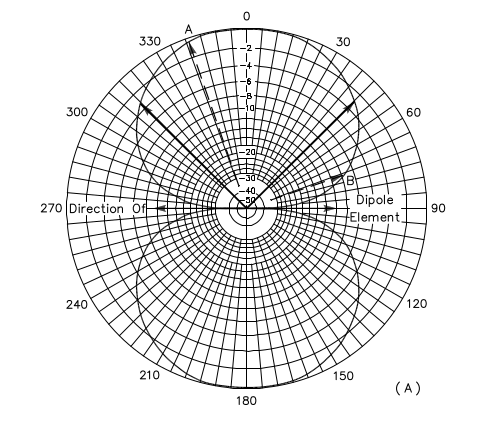
\includegraphics[width=6cm]{radiatingPatternDipole1}
    % \caption{Esquemático del modulador.}
  \end{subfigure}
  \begin{subfigure}[b]{0.4\textwidth}
    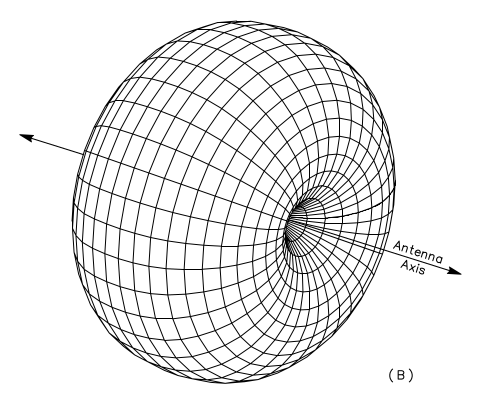
\includegraphics[width=6cm]{radiatingPatternDipole2}
    % \caption{PCB del modulador.}
  \end{subfigure}             
  \caption{Diagrama de radiación de un dipolo \cite{arrl2007}.}
  \label{fig:radingPatternDipole}
\end{figure}

La directividad de un monopolo de cuarto de longitud de onda es el doble que el un dipolo de media longitud de onda en espacio libre \cite{Stutzman2013},
\begin{equation}
  D = 2(1.64) = 3.28 = \SI{5.16}{\dB}
\end{equation}

La impedancia de entrada de un monopolo de un cuarto de longitud de onda infinitesimalmente fino resulta \cite{Stutzman2013},
\begin{equation}
  \bm{Z} = ~ (72 + j42.5) = 36 + j\SI{21.3}{\Omega}
\end{equation}

\subsection{Polarización} \label{sc:polarization}

La polarización de una onda radiada se la define como la propiedad de una onda electromagnética describiendo la variación en tiempo de la dirección y la magnitud relativa del vector del campo eléctrico; específicamente, la figura trazada en función del tiempo por la extremidad del vector en un lugar fijo en el espacio, y el sentido en que es trazado, como observado a lo largo de la dirección de propagación. Por lo tanto, la polarización es la curva trazada por la punta del vector que representa el campo eléctrico instantáneo \cite{Balanis2012}.

La polarización se puede clasificar como lineal, circular o elíptica (ver figura \ref{fig:hvPolarizations}). Si el vector que describe el campo eléctrico en un punto del espacio en función del tiempo recorre un trayecto a lo largo de una línea, se dice que el campo es linealmente polarizado (horizontalmente y/o verticalmente). En general, la figura trazada por el campo eléctrico es una elipse, nombrada polarización elíptica. La polarización lineal y circular son casos especiales de la elíptica \cite{Vita2012}.

\begin{figure}[H]
  \centering
  \begin{subfigure}[b]{0.49\textwidth}
    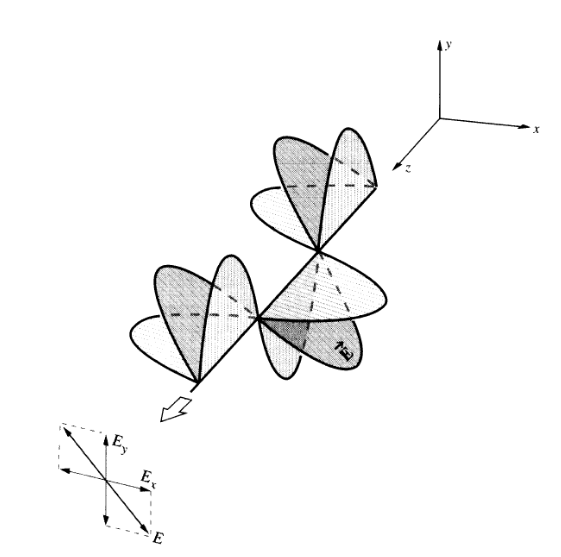
\includegraphics[width=7cm]{linearPolarization}
    \caption{Polarización lineal.}
  \end{subfigure}
  \begin{subfigure}[b]{0.49\textwidth}
    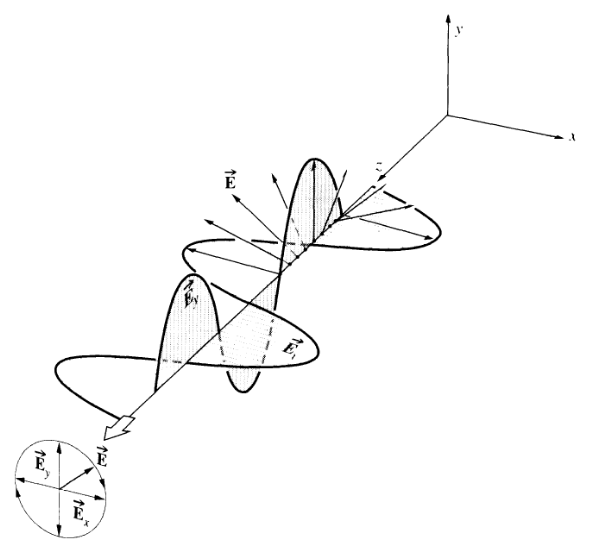
\includegraphics[width=7cm]{circularPolarization}
    \caption{Polarización circular.}
  \end{subfigure}
  \caption{Distintos tipos de polarizaciones \cite{Hecht2002}.}
  \label{fig:hvPolarizations}
\end{figure}

Para el caso de esta tesis, las antenas a construir son polarimétricas. Esto implica que poseen dos componentes, una Horizontal (H) y otra Vertical (V). Con esto se define el requerimiento \ref{req:l2_polarization}.


\section{Parámetros S} 

La sigla S deriva de la palabra dispersión. Para altas frecuencias, es conveniente describir una determinada red en términos de ondas en vez de tensiones o corrientes. Esto permite una definición más sencilla de planos de referencia. Por razones prácticas, la descripción en términos de ondas entrantes y salientes ha sido introducida. Ahora, una red de 4 polos se transforma en 2 puertos y $2n$ polos se transforman en $n$ puertos. En el caso de un número impar de polos (ej. 3 polos), un punto de referencia puede ser elegido, atribuyendo un polo igualmente a dos puertos. Por lo tanto 3 polos se convierten en 3 + 1 polo correspondiendo a 2 puertos. Como una regla general, para cantidades impares de polos, siempre se agrega un polo extra \cite{Caspers}.

\begin{figure}[H]
 \centering
 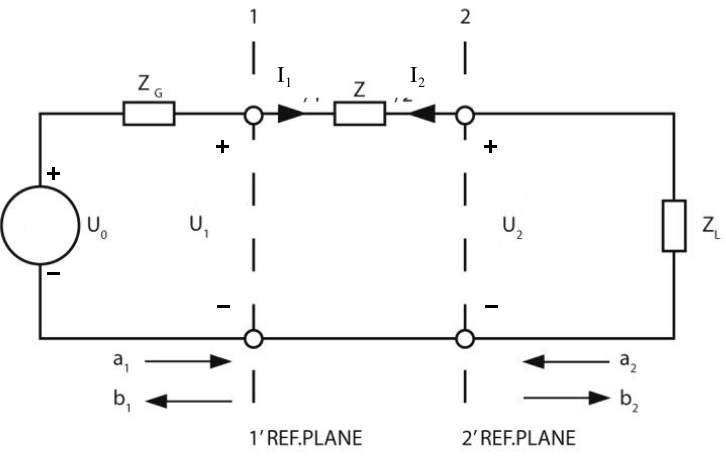
\includegraphics[width=10cm]{sParameters1}
 \caption{Ejemplo de una red de 2 puertos: circuito serie \cite{Caspers}}
 \label{fig:esquema_serie}
\end{figure}

Tomando como ejemplo una red de 2 puertos compuesta por una sola impedancia $\bm{Z}$ conectada en serie (figura \ref{fig:esquema_serie}). Las impedancias de la fuente y de la carga son $\bm{Z_G}$ y $\bm{Z_L}$ respectivamente. Si $\bm{Z}=0$ y $\bm{Z_L} = \bm{Z_G}$ (para el caso de $\bm{Z_G}$ real) la carga está adaptada. En este caso se obtiene una máxima transferencia de potencia y $\bm{U_1} = \bm{U_2} = \bm{U_0}/2$. Notar que todas las tensiones y corrientes son valores pico. Se supone que las líneas que unen los componentes poseen longitud eléctrica igual a 0. Las conexiones con una longitud eléctrica finita están dibujadas como una doble línea. A continuación se relacionará $\bm{U_0}$, $\bm{U_1}$ y $\bm{U_2}$ a $\bm{a}$ y $\bm{b}$.


\subsection{Definición de "ondas de potencia"}

Las ondas incidentes al puerto son $\textbf{a}=(\bm{a_1}, \bm{a_2}, \bm{a_3}, ..., \bm{a_n})$, las ondas salientes, o reflejadas, del puerto son $\textbf{b}=(\bm{b_1}, \bm{b_2}, \bm{b_3}, ..., \bm{b_n})$. Por definición, las corrientes incidentes son positivas y las salientes negativas. La onda $\bm{a_1}$, incidente al puerto 1, es derivada de la tensión entrante a la carga balanceada.

Para hacer que ésta definición sea consistente con la ley de la conservación de la energía. La tensión es normalizada a $\sqrt{\bm{Z_0}}$. $\bm{Z_0}$ es, en general una impedancia de referencia arbitraria, que usualmente se la utiliza como la impedancia característica de la línea (ej, $\bm{Z_0} = 50 \Omega$). Y, cuando todas las impedancias son iguales ($\bm{Z_G} = \bm{Z_L} = \bm{Z_0}$), se dice que la línea está adaptada y no hay onda reflejada. Las definiciones de $\bm{a_1}$ y $\bm{b_1}$ son
\begin{equation}
\begin{aligned}
  \bm{a_1} &= \dfrac{\bm{U_0}}{2\sqrt{\bm{Z_0}}}= \dfrac{\textrm{onda de tensión incidente (puerto 1)}}{\sqrt{\bm{Z_0}}}=\dfrac{\bm{U_1}^{inc}}{\sqrt{\bm{Z_0}}} \\
  \bm{b_1} &= \dfrac{\bm{U_1}^{refl}}{2\sqrt{\bm{Z_0}}}= \dfrac{\textrm{onda de tensión reflejada (puerto 1)}}{\sqrt{\bm{Z_0}}}
\end{aligned}
\end{equation}

Notar que \textbf{a} y \textbf{b} tienen las unidades de $\sqrt{\textrm{potencia}}$.

La potencia incidente al puerto 1, $P_{inc}$, es simplemente la potencia entregada por la fuente, mientras que la potencia saliente del puerto 1, $P_{refl}$, viene de la onda de tensión reflejada.
\begin{equation}
\begin{aligned}
  P_1^{inc} &= \dfrac{1}{2}|\bm{a_1}|^2= \dfrac{|\bm{U_1}^{inc}|^2}{2\bm{Z_0}}=\dfrac{|\bm{I_1}^{inc}|^2}{2}\bm{Z_0} \\
  P_1^{refl} &= \dfrac{1}{2}|\bm{b_1}|^2= \dfrac{|\bm{U_1}^{refl}|^2}{2\bm{Z_0}}=\dfrac{|\bm{I_1}^{refl}|^2}{2}\bm{Z_0} \\
\end{aligned}
\end{equation}

En el caso de una desadaptación de la impedancia de carga $\bm{Z_L}$, parte de la potencia será reflejada a través del puerto 2 (potencia incidente al puerto 2).
\begin{equation}
P_2^{inc}=\dfrac{1}{2}|\bm{a_2}|^2
\end{equation}

Se ha definido $\bm{a_1} = \bm{U_0}/2\sqrt{\bm{Z_0}} = \bm{U}^{inc}/\sqrt{\bm{Z_0}}$ con la onda de tensión incidente $\bm{U}^{inc}$. Como analogía se la puede definir como $\bm{a_1} = \bm{I}^{inc}\sqrt{\bm{Z_0}}$ con la onda incidente de corriente $\bm{I}^{inc}$. Utilizando ambas, se obtiene la definición general de las ondas incidentes $\bm{a_i}$ y reflejadas $\bm{b_i}$ de un puerto.
\begin{equation}
\begin{aligned}
  \bm{a_i} &= \dfrac{\bm{U_i} + \bm{I_i}\bm{Z_0}}{2\sqrt{\bm{Z_0}}} \\
  \bm{b_i} &= \dfrac{\bm{U_i} - \bm{I_i}\bm{Z_0}}{2\sqrt{\bm{Z_0}}}
\end{aligned}
\label{eq:waves}
\end{equation}

Solucionando este sistema de ecuaciones, $\bm{U_i}$ y $\bm{I_i}$ pueden ser obtenidas de $\bm{a_i}$ y $\bm{b_i}$ como
\begin{equation}
\begin{aligned}
  \bm{U_i} &= \sqrt{\bm{Z_0}}(\bm{a_i} + \bm{b_i}) = \bm{U_i}^{inc} + \bm{U_i}^{refl}\\
  \bm{I_i} &= \dfrac{1}{\sqrt{\bm{Z_0}}}(\bm{a_i} - \bm{b_i}) = \dfrac{\bm{U_i}^{refl}}{\bm{Z_0}}
\end{aligned}
\end{equation}


\subsection{La matriz de parámetros S}

La relación entre $\bm{a_i}$ y $\bm{b_i}$ (siendo $i=1..n$) puede ser escrito como un sistema de n ecuaciones lineales (siendo la variable independiente $\bm{a_i}$ y $\bm{b_i}$ la dependiente)
\begin{equation}
\begin{aligned}
  \bm{b_1} = \bm{S}_{11}\bm{a_1} + \bm{S}_{12}\bm{a_2} \\
  \bm{b_2} = \bm{S}_{21}\bm{a_1} + \bm{S}_{22}\bm{a_2}
\end{aligned}
\label{eq:s_matrix}
\end{equation}

Escrito de forma matricial: \textbf{b} = \textbf{Sa}

El significado físico de los parámetros S es:
\begin{itemize}
  \item $\bm{S}_{11}$: es el coeficiente de reflexión con la salida de la red terminada en una carga adaptada ($\bm{a_2} = 0$).
  \item $\bm{S}_{21}$: es la transmisión en directa (del puerto 1 al 2)
  \item $\bm{S}_{12}$: es la transmisión en inversa (del puerto 2 al 1)
  \item $\bm{S}_{22}$: es el coeficiente de reflexión de la salida.
\end{itemize}

Al medir todos los parámetros S de una red de n puertos, todos los puertos deben estar terminados con una carga adaptada. Utilizando las ecuaciones \ref{eq:waves} y \ref{eq:s_matrix} se obtiene el coeficiente de reflexión de una impedancia $\bm{Z_L}$ conectada a un generador de impedancia de salida $\bm{Z_0}$ (Figura \ref{fig:esquema_serie}, caso $\bm{Z_G} = \bm{Z_0}$ y $\bm{Z} = 0$)
\begin{equation}
\bm{S}_{11} = \dfrac{\bm{b_1}}{\bm{a_1}}\bigg|_{\bm{a_2}=0} = \dfrac{\bm{U_1} - \bm{I_1}\bm{Z_0}}{\bm{U_1} + \bm{I_1}\bm{Z_0}} = \dfrac{\bm{Z_L} - \bm{Z_0}}{\bm{Z_L} + \bm{Z_0}} = \bm{\Gamma}
\end{equation}


\section{Procesamiento de la señal de un radar FMCW}

Hay distintos tipos de modulaciones con las que se puede transmitir utilizando dicho tipo de radar, las cuales están resumidas a continuación.

\begin{description}

\item[Modulación diente de sierra] En esta modulación se transmite una rampa en frecuencia con respecto al tiempo y es utilizada para distancias grandes combinado con una influencia despreciable de frecuencia doppler. Si se observara un blanco estático, el eco recibido solamente posee un desplazamiento en tiempo, en cambio, si está en movimiento se genera una frecuencia doppler. Dicho efecto desplaza la frecuencia de la señal recibida incrementándola, si el blanco se mueve hacia el radar, o decrementándola, si se aleja del mismo. En esta modulación el receptor no tiene forma de separar ambas frecuencias, por lo tanto, el efecto doppler es tomado como un error en la medición. Un ejemplo es un radar de navegación marítimo \cite{Basics2015}. En \cite{Varavin2007a, Shen} se detalla el procesamiento de este tipo de modulación para un radar FMCW.

\item[Modulación Triangular] En un cambio de frecuencia de forma triangular, se pueden utilizar ambas pendientes para medir la distancia al cuerpo. Sin efecto doppler, el desplazamiento en tiempo del eco, por ende la diferencia en frecuencia es la misma tanto para la pendiente positiva como negativa. En cambio, como el efecto doppler incrementa o decrementa las frecuencias del eco, en una de las pendientes la diferencia de frecuencias se aumenta, pero para la otra decrece en la misma medida. Haciendo un análisis y comparando los resultados de cada pendiente de forma separada, se permite determinar fácilmente la diferencia en frecuencia $\Delta f$ con respecto a la frecuencia doppler $f_D$ \cite{Basics2015}. En \cite{Chang2006, Kurt2007} se detalla el procesamiento de este tipo de modulación para un radar FMCW.

\item[Modulación cuadrada o FSK] Esta modulación es utilizada para mediciones muy precisas de rango a distancias cortas. Se compara la fase de la señal recibida de las distintas frecuencias transmitidas. La mayor desventaja es que no se puede distinguir los ecos de distintos blancos iluminados y que el rango sin ambigüedades es muy chico \cite{Basics2015}.

\item[Modulación escalonada] Para detectar objetos con un mucho ruido del entorno, o clutter, para la distinción del objeto requiere alta resolución en rango. Esto se obtiene utilizando pulsos cortos y de gran ancho de banda, por lo tanto, se debe utilizar un receptor de gran ancho de banda, el cual es muy costoso. Para no utilizar un receptor de gran ancho de banda, se modula la frecuencia de forma escalonada en sucesivos pulsos, de esta forma, la resolución en rango no se ve comprometida \cite{steppedFreq}. A su vez, esta modulación se la utiliza para mediciones de interferometría y aumenta el rango de mediciones sin ambigüedades \cite{Basics2015}.

Es importante destacar que las señales que poseen una modulación del tipo rampa son llamadas chirps.

\end{description}

En esta tesis se utiliza la modulación diente de sierra dado que el radar es utilizado para realizar mediciones con blancos estáticos. De esta forma se define el requerimiento \ref{req:l2_mod}. La figura \ref{fig:sawtoothSignal} ilustra para un caso general los parámetros que definen dicha señal, los cuales son el ancho de banda de la señal transmitida ($BW$) y el período ($T$) o tiempo de repetición de dicho pulso ($PRT$).

\begin{figure}
 \centering
 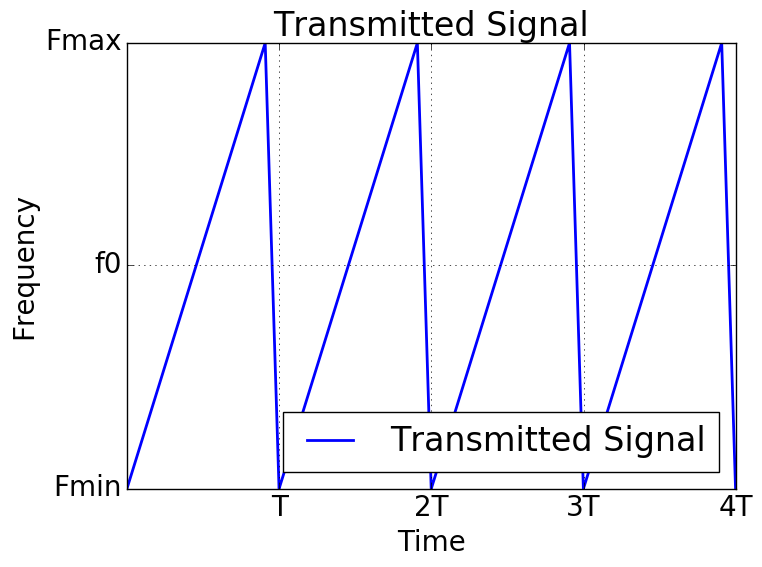
\includegraphics[width=10cm]{sawtoothSignal}
 \caption{Modulación diente de sierra de la señal a transmitir.}
 \label{fig:sawtoothSignal}
\end{figure}

Para extraer el efecto que el medio induce sobre la señal, es importante saber determinar la distancia a la cual está el cuerpo iluminado con respecto al radar. De esta forma se define el requerimiento \ref{req:l1_distance}. Para el desarrollo a continuación se asume que se está trabajando en campo lejano, con esta suposición el campo eléctrico y magnético de la onda transmitida y recibida son ortogonales a la dirección de la misma. En general, cuando se está a unas pocas longitudes de onda de distancia ya se cumple esta condición. En un monopolo se cumple a una distancia $r$ aproximadamente igual a $\lambda/ 6$ \cite{Richards2009}.


\subsection{Determinación de distancia}

Para determinar la distancia de un cuerpo iluminado se mide el tiempo de ida y vuelta de la señal transmitida. En la figura \ref{fig:roundTripTime} se muestra la modulación de una chirp transmitida por el radar y el eco recibido, producido por dicho blanco a una distancia $R$. Se puede observar que el tiempo de ida y vuelta de la señal está marcado como $\tau$.

\begin{figure}
 \centering
 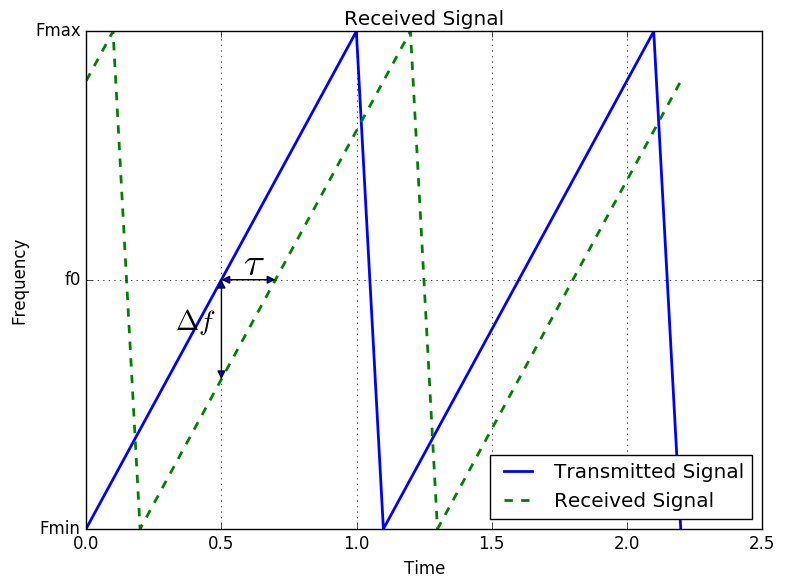
\includegraphics[width=10cm]{round-tripTime}
 \caption{Modulación diente de sierra de la señal a transmitir.}
 \label{fig:roundTripTime}
\end{figure}

La relación entre el tiempo de ida y vuelta $\tau$ y la distancia es,
\begin{equation}\label{eq:relDist}
  \tau = \dfrac{2R\sqrt{\varepsilon_r}}{c}
\end{equation}
donde $\varepsilon_r$ es la permitividad relativa del medio.

Este tipo de radares utiliza la relación entre la diferencia de tiempo $\tau$ y la diferencia en frecuencia, $\Delta f$, entre las señales transmitidas y recibidas,
\begin{equation}\label{eq:relFreqDist}
  \tau = \dfrac{T\Delta f}{B}
\end{equation}
donde $B$ es el ancho de banda de la señal y $T$ es el tiempo en que es barrido el BW, desde la frecuencia mínima a la máxima, sin contar el tiempo que tarda el generador en volver de la frecuencia máxima a la mínima. Por lo tanto utilizando las ecuaciones \ref{eq:relDist} y \ref{eq:relFreqDist} se puede determinar la distancia $R$ a partir de la señal recibida,
\begin{equation}\label{eq:receivedDist}
  R = \dfrac{T\Delta fc}{2B\varepsilon_r}
\end{equation}

Para determinar la resolución en distancia, se debe tener en cuenta que la misma está relacionada con la resolución espectral de la señal recibida. Asumiendo $T >> T_d$, el ancho de banda a $\SI{-3}{\dB}$ con respecto a su pico es igual a $1/T$ \cite{Brooker2005}. Es importante destacar que dicho valor es igual a la distancia entre las frecuencias nulas, dado que el espectro se corresponde a una sinc.
\begin{equation}\label{eq:resolutionDistance}
  \Delta R = \dfrac{c}{2B\sqrt{\varepsilon_r}}
\end{equation}

Se puede apreciar que la resolución en distancia obtenida, ecuación \ref{eq:resolutionDistance}, no depende ni del período ($T$) de la señal transmitida ni de su frecuencia central ($f_0$), solamente de su ancho de banda ($B$). Hay que tener en cuenta que las alinelidades de la señal modulada degradan la resolución obtenida, y la misma depende del ancho de banda, por lo tanto, la mayor resolución se obtiene tomando en cuenta ambos efectos \cite{Brooker2005}.

Como la distancia al cuerpo se determina midiendo la frecuencia de la señal recibida, o en su defecto el pico de la sinc en frecuencia, se pueden agregar ceros al final de la señal para aumentar la resolución de la FFT. Dicho proceso es llamado zero padding \cite{Oppenheim1990}.
\begin{equation}\label{eq:resolutionDistance2}
  \Delta R = \dfrac{c}{2B\sqrt{\varepsilon_r}p}
\end{equation}

Siendo $p$ la relación entre la frecuencia de muestreo $f$ de la señal y la cantidad de muestras $n$ utilizada para realizar la FFT.
\begin{equation}
  p = \frac{f}{n}
\end{equation}


\subsection{Determinación de la relación de fase}

Para determinar la fase del cuerpo iluminado es necesario realizar un análisis de la fase de la señal recibida. La figura \ref{fig:phaseSystem} muestra el recorrido de la señal, en particular centrando en el análisis que se está realizando.
\begin{figure}[htb]
 \centering
 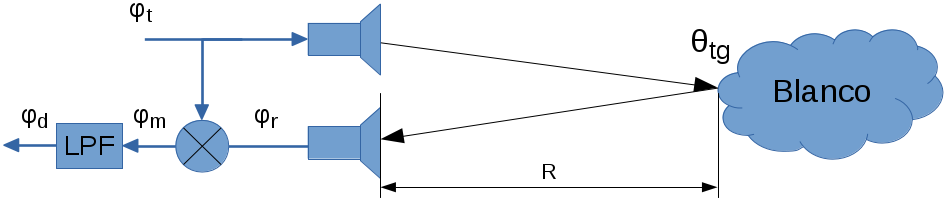
\includegraphics[width=10cm]{phaseMeasurement}
 \caption{Análisis de fase del sistema completo.}
 \label{fig:phaseSystem}
\end{figure}

La ecuación que define la modulación de cada período del pulso se encuentra descripta a continuación,
\begin{equation}
  f(t) = f_0 + \dfrac{B}{T}(t-\dfrac{T}{2}),\quad 0 \le t < T
  \label{eq:signalFrequency}
\end{equation}

donde $c$ es la velocidad de la luz, $\varepsilon_r$ es la constante dieléctrica del medio \cite{Brennan2014a} y $T$ es el tiempo en que es barrido el BW, desde la frecuencia mínima a la máxima, sin contar el tiempo que tarda el generador en volver de la frecuencia máxima a la mínima. Dado que la fase de una señal es la integral de su frecuencia sumada a una constante, se obtiene la fase instantánea transmitida a partir de la ecuación \ref{eq:signalFrequency},
\begin{equation}
  \varphi_t(t) = 2\pi f_0t + \dfrac{2\pi B}{2T}(t^2-Tt) + \phi_0,\quad 0 \le t < T
  \label{eq:signalFrequency2}
\end{equation}

El eco recibido por un objeto puntual en una distancia $R$ y desfasando la señal en $\theta$ llega al radar con la fase,
\begin{equation}
  \varphi_r(t) = w_0(t-\tau) + \dfrac{2\pi B}{2T}((t - \tau)^2-T(t - \tau)) + \theta + \phi_0,\quad 0 \le t < T
  \label{eq:signalFrequency3}
\end{equation}

donde $\tau$ es el tiempo ida y vuelta de la señal entre el transmisor y receptor del radar obtenido de la ecuación \ref{eq:relDist}.

Luego, en el mezclador, la señal recibida se la multiplica con la transmitida, por identidad trigonométrica, se obtiene
\begin{equation}
  x_m(t) = \dfrac{A_tA_r}{2}(\cos(\varphi_t(t)+\varphi_r(t)) + \cos(\varphi_t(t)- \varphi_r(r)))
  \label{eq:signalFrequency4}
\end{equation}

Donde $A_r$ es la amplitud de la señal recibida, la cual es modificada por el ida y vuelta del medio y por el blanco donde se genera el eco de la señal.

Que, luego del filtro pasa bajos, el primer término de la ecuación \ref{eq:signalFrequency4}, el cual posee una frecuencia de $2w_0$, resulta completamente atenuado, quedando solamente el término con la resta de fases,
\begin{equation}
  x_d(t) = \dfrac{A_tA_r}{2}\cos(w_0\tau + \dfrac{2\pi B\tau}{T}(t - \dfrac{T}{2}) - \dfrac{2\pi B\tau^2}{2T} - \theta)
  \label{eq:signalFrequency5}
\end{equation}

Es importante notar que la fase inicial de transmisión se elimina, por lo tanto no importa cual es la fase inicial de cada pulso
transmitido ni su variación entre pulsos. Para determinar la frecuencia de la señal recibida se deriva la ecuación \ref{eq:signalFrequency5}, 
\begin{equation}\label{eq:beatFreq}
  w_d = \dfrac{2\pi B\tau}{T} \rightarrow f_d = \dfrac{B\tau}{T}
\end{equation}

Se puede observar que el resultado obtenido es coherente con el resultado de la ecuación \ref{eq:relFreqDist}, el cual muestra la relación entre el round-trip time y la diferencia en frecuencia entre la señal transmitida y recibida.

Del resultado de la ecuación \ref{eq:signalFrequency5} se observa que la fase de la señal recibida está compuesta por cuatro términos.
\begin{itemize}
  \item $w_0\tau$ es el término utilizado para determinar distancias con alta precisión en blancos conocidos \cite{Brennan2014a}.
  \item $\dfrac{2\pi B\tau}{T}(t - \dfrac{T}{2})$ es un término de fase lineal con el tiempo que representa la frecuencia de la señal.
  \item $\dfrac{2\pi B\tau^2}{2T}$ es un offset en la señal, usualmente pequeño.
  \item $\theta$ es el término de fase originada por el blanco donde incidió la señal transmitida por el radar.
\end{itemize}

Para obtener el término de la fase originada por el blanco, $\theta$, primero se calcula la FFT de la señal recibida y se mide la fase del pico de la sinc, $\varphi_d$. Si no se realiza ninguna rotación a la señal en el momento del cálculo, el valor de $t$ correspondiente al segundo término es igual a 0. Luego, se debe restar dicho valor a la fase de los primeros tres términos correspondientes a la la distancia medida, 
\begin{equation}\label{eq:phaseMeasurement}
  \theta =  w_0\tau - \pi B\tau - \dfrac{\pi B\tau^2}{T} - \varphi_d  = \dfrac{2w_0R}{c} - \dfrac{2\pi BR}{c} - \dfrac{4\pi BR^2}{Tc^2} - \varphi_d
\end{equation}

Para utilizar la ecuación anterior, es fundamental que la diferencia de fase entre dos pulsos consecutivos en frecuencia sea menor que $2\pi$. Para ello, se realiza zero padding en la señal previo al cálculo de la FFT.

% Si se quisiera utilizar $w_0\tau$ para calcular la distancia, primero se tiene que hacer zero padding en la señal (para calcular la frecuencia de round trip time) de manera tal que la diferencia de fase entre dos pulsos consecutivos en frecuencia (que estan totalmente relacionados a $\Delta R$) sea menor que $2\pi$. Con esto, el $\Delta R$ al que está relacionado el pico de frecuencia entre dichos pulsos se puede determinar univocamente. La relación entre la fase y dicha distancia es $\Delta R = \frac{\lambda\phi}{4\pi}$, está dividido por 4 porque la distancia medida es el doble a la distancia entre el radar y el obteto iluminado.

% Sabiendo que la relación entre la distancia y la frecuencia medida, expresada en \ref{eq:beatFreq}, la máxima diferencia de distancia en que puede estar el objeto iluminado es igual a $\Delta R = \frac{c}{2B\sqrt{\varepsilon_r}}$, $\Delta f_d = \frac{1}{T}$ dado que es la resolución el frecuencia. Por lo tanto, la diferencia de fase es.

% \begin{equation}
%   \Delta(\omega_0\tau) = \dfrac{\omega_02\Delta R \sqrt{\varepsilon_r}}{c} = \dfrac{\omega_c}{B} = \dfrac{2\pi f_0}{B}
% \end{equation}


% \mynote{however, the phase indicated by an FFT is that at the start of the sample, at t = 0. It is therefore necessary to rotate the deramped (time-domain) waveform so that the centre of the waveform aligns with the start of the sample, t = 0, prior to FFT processing \cite{Brennan2014a}}

% \mynote{For processing convenience, it would be highly desirable if
% the phase relating to a point target located at the centre of each range bin is normalised to zero. This can be achieved by weighting the FFT-processed deramped waveform by a reference array equal to the phase conjugate of the expected phase at the centre of each range bin}

% \mynote{Seleccionar una función de ventana no es una tarea simple. Cada función de ventana tiene sus propias características y aptitud para diferentes aplicaciones. Para elegir una función de ventana, usted debe calcular el contenido de la frecuencia de la señal.
% Si la señal contiene componentes de frecuencia de fuerte interferencia alejados de la frecuencia de interés, elija una ventana con un rango alto de caída del lóbulo lateral.
% Si la señal contiene fuertes señales de interferencia cerca de la frecuencia de interés, elija una función de ventana con un nivel bajo de lóbulo lateral máximo.
% Si la frecuencia de interés contiene dos o más señales muy cerca una de la otra, la resolución espectral es importante. En este caso, es mejor elegir una ventana con un lóbulo principal muy estrecho.
% Si la precisión de la amplitud de un solo componente de frecuencia es más importante que la ubicación exacta del componente en un contenedor de frecuencia determinado, elija una ventana con un lóbulo principal amplio.
% Si el espectro de la señal es más bien plano o de banda ancha en el contenido de frecuencia, utilice la ventana uniforme o ninguna ventana.
% En general, la ventana Hanning (Hann) es satisfactoria en el 95\% de los casos. Tiene buena resolución de frecuencia y menor fuga espectral. Si no conoce la naturaleza de la señal, pero desea aplicar una ventana, comience con la ventana de Hann.
% http://www.ni.com/white-paper/4844/es/}


% \mynote{el mismo libro \cite{Richards2009} tiene una buena definicion con un buen grafico de polarización.}

\subsection{Determinación de la relación de amplitud}


Para determinar la ganancia del blanco, se debe realizar un análisis de potencia en todo el sistema, el cual se ilustra en la figura  \ref{fig:powerAnalysis}. Se puede observar que la señal transmitida posee atenuaciones por el medio en que la señal es transmitida y recibida, el blanco, las ganancias de transmisión y recepción de las antenas, el mezclador del receptor y el filtro pasa bajos. 

\begin{figure}
 \centering
 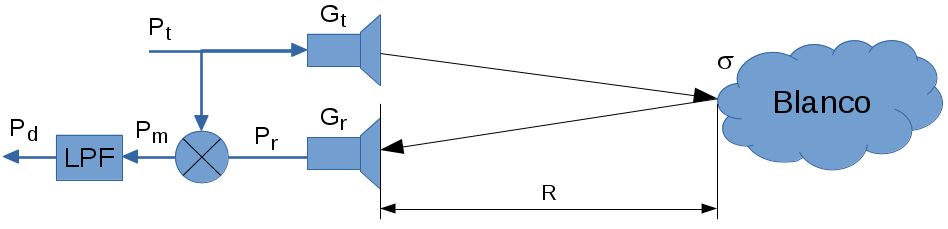
\includegraphics[width=10cm]{targetMeasurement}
 \caption{Análisis de la potencia de la señal.}
 \label{fig:powerAnalysis}
\end{figure}

Cuando el radar transmite una potencia $P_t$ y si fuese un radiador isotrópico, la densidad de potencia incidente en un cuerpo a una distancia R es igual a $P_t$ dividido el área unitaria,
\begin{equation}
  p_i = \dfrac{P_t}{4\pi R^2} \,[\si{Wm^{-2}}]
\end{equation}

Cuando el radiador no es isotrópico y el radar utiliza una antena que concentra la potencia en una dirección en particular, la densidad de potencia incidente resulta
\begin{equation}
  p_i = \dfrac{P_tG_t}{4\pi R^2} \,[\si{Wm^{-2}}]
\end{equation}

donde $G_t$ es la ganancia de la antena transmisora, definida como la relación entre densidades de potencia en la dirección en particular con respecto a un radiador isotrópico \cite{Richards2009}. Ahora, si se asume que el blanco posee un Radar Cross Section (RCS) igual a $\sigma \,[\si{m^2}]$, la potencia disponible para ser nuevamente irradiada en el blanco es 
\begin{equation}
  p_\sigma = p_i\sigma = \dfrac{P_tG_t\sigma}{4\pi R^2} \,[\si{W}]
\end{equation}

A su vez, si se asume que el blanco irradia isotrópicamente, la densidad de potencia en la antena receptora es 
\begin{equation} \label{eq:receivedDensity}
  p_r = \dfrac{P_tG_t\sigma}{(4\pi)^2 R^4} \,[\si{Wm^{-2}}]
\end{equation}

La potencia recibida es la densidad multiplicada por la apertura de la antena $A_r$, que también tiene dimensiones de área. La cual está relacionada con la ganancia de recepción por 
\begin{equation} \label{eq:receptionGain}
  G_r = \dfrac{4\pi A_r}{\lambda^2}
\end{equation}

Por lo tanto, utilizando la ecuación \ref{eq:receivedDensity} con \ref{eq:receptionGain}, la potencia recibida $P_r$ por el radar es igual a
\begin{equation}
  P_r = \dfrac{P_tG_tG_r\lambda^2\sigma}{(4\pi)^3 R^4} \,[\si{W}]
\end{equation}

La señal recibida es mezclada con la señal transmita y, si se asume un mezclador ideal, la potencia de salida $P_m$ es la multiplicación de las potencias de entrada, por lo tanto
\begin{equation}
  P_m = P_tP_r = \dfrac{P_t^2G_tG_r\lambda^2\sigma}{(4\pi)^3 R^4} \,[\si{W}]
\end{equation}

Por último, la señal mezclada es filtrada eliminando los componentes de alta frecuencia, asumiendo un filtro ideal y observando que en la ecuación \ref{eq:signalFrequency4} se elimina el término correspondiente a la suma de frecuencias, se puede deducir que la potencia de salida es la mitad que la de entrada.
\begin{equation} \label{eq:derampedPower}
  P_d = \dfrac{P_m}{2} = \dfrac{P_t^2G_tG_r\lambda^2\sigma}{2(4\pi)^3 R^4} \,[\si{W}]
\end{equation}

Ahora que se posee la relación entre la potencia de la señal a procesar y la ganancia del blanco (ecuación \ref{eq:derampedPower}), se puede determinar la relación de amplitud
\begin{equation}
  \sigma = \dfrac{2P_d(4\pi)^3 R^4}{P_t^2G_tG_r\lambda^2} \,[\si{m^2}]
\end{equation}


\section{Resumen}

En este capítulo se introdujeron los conceptos básicos sobre los dos grandes grupos de radares, los cuales son pulsados o continuos y se menciona la problemática de ambigüedades en rango asociada a cada uno de ellos. En la problemática a resolver se opta por la utilización de radares continuos a causa de la cercanía entre el blanco y el radar.

Con respecto a las antenas, se menciona una lista de los distintos tipos con descripciones y usos. Se detallan los monopolos y dipolos dado que es el tipo de antena utilizado por su simpleza de construcción. A su vez, se introduce el concepto de parámetros S y de polarización vertical y horizontal dado que las antenas utilizadas son del tipo polarimétricas y se las caracteriza midiendo dichos parámetros.

Por último, se resumen los principales tipos de modulaciones utilizados en un radar continuo detallando el diente de sierra. Asimismo, se describe el desarrollo matemático para la determinación de la distancia entre el objeto y el radar. Esto es necesario dado que la misma es utilizada para poder determinar tanto la fase como la ganancia que el blanco induce sobre la señal. Dichas perturbaciones son las variables que determinan los parámetros de dispersión.

\begin{description}

\item[Distancia entre el blanco y el radar]
Dicha variable está determinada por
\begin{equation}
  R = \dfrac{T\Delta fc}{2B\varepsilon_r} \pm \dfrac{c}{2B\sqrt{\varepsilon_r}p}
\end{equation}
donde $c$ es la velocidad de la luz, $\varepsilon_r$ es la permitividad relativa del medio, $B$ es el ancho de banda de la señal, $\Delta f$ es la diferencia de frecuencia instantánea entre la señal transmitida y recibida, $T$ es el tiempo en que es barrido el BW, desde la frecuencia mínima a la máxima y $p$ es la relación entre la frecuencia de muestreo de la señal y la cantidad de muestras utilizada para realizar la FFT.

\item[Atenuación que el blanco induce sobre la señal]
Dicha variable está determinada por
\begin{equation}
  \sigma = \dfrac{2P_d(4\pi)^3 R^4}{P_t^2G_tG_r\lambda^2}
\end{equation}
donde $P_d$ es la potencia de la señal a procesar, $P_t$ es la potencia transmitida del radar, $G_t$ es la ganancia de la antena transmisora y $G_r$ es la ganancia de la antena receptora.

\item[Desfase que el blanco induce sobre la señal]
Dicha variable está determinada por
\begin{equation}
  \theta = \dfrac{4\pi f_0R}{c} - \dfrac{2\pi BR}{c} - \dfrac{4\pi BR^2}{Tc^2} - \varphi_d
\end{equation}
donde $f_0$ es la frecuencia central de la señal transmitida y $\varphi_d$ es la fase de de la señal recibida.

Para utilizar la ecuación anterior, es fundamental que la diferencia de fase entre dos pulsos consecutivos en frecuencia sea menor que $2\pi$. Para ello, se realiza zero padding en la señal previo al cálculo de la FFT.
\end{description}